\documentclass{beamer}
%\documentclass[UTF8]{ctexbeamer} % Chines Version
\usepackage{xifthen}
\usepackage[utf8]{inputenc}
\usepackage{utopia}            % font utopia imported
\usepackage{amsmath}
\usepackage{latexsym}
\usepackage{calc}              % support command '\widthof'
\usepackage{xcolor}            % support multiple color 
\usepackage{arydshln}
\usepackage{amssymb}  
\usepackage{booktabs}
\usepackage{graphicx}
\usepackage{subcaption}
\usepackage{bookmark}
\usepackage{float}
\usepackage{bm}
\usepackage{bbold}
\usepackage{extarrows}
\usepackage{ctex, xeCJK, zxjatype}


%--------
\usepackage{listings}
\usepackage{xcolor}
\usepackage{xparse}
% \usepackage{etoolbox}
% \NewDocumentCommand\cfig{om}{%
%   \IfNoValueF{#1}{(((#1)))}%
% }
\newcommand{\cfig}[2]{
    \begin{figure}[htbp]
    \centering
    \includegraphics[width=#2\textwidth]{#1}
\end{figure}
}

\newcommand{\R}{\mathbb{R}}
\newcommand{\bt}[1]{\textbf{#1}}
\newcommand{\bs}[1]{\boldsymbol{#1}}

\newenvironment{remark}[1][Remark]{\begin{trivlist}
    \item[\hskip \labelsep {\bfseries #1}]}{\end{trivlist}}


\usefonttheme{professionalfonts} 

\makeatletter
\let\@@magyar@captionfix\relax
\makeatother

\usetheme{Madrid}
% \usetheme{Singapore}
% \usetheme{Pittsburgh}
%\usecolortheme{default,beaver,lily,orchid,seahorse} 
\usecolortheme{default}
%default、albatross、beaver、beetle、crane、dolphine、dove、fly、lily、orchid、rose、seagull、seahorse、sidebartab、structure、whale、wolverine

%======================================================================%
\title[PKUAI]{Recent VQA Approaches}

%\subtitle{(To throw out a brick to attract a jade)}

\author[Wentao Mo]
{Wentao Mo\inst{1}}  

\institute[AI@PKU] 
{
    \inst{1}%
    Department of Machine Intelligence\\
    Peking University
}

\date[PKU]{\today}
%======================================================================

%======================================================================
% \AtBeginSection[]
% {
% \begin{frame}
%     \frametitle{Outline}
%     \tableofcontents[currentsection]
% \end{frame} 
% }
%======================================================================

\begin{document}
%======================================================================
\frame{\titlepage}
%======================================================================

%======================================================================
\begin{frame}
    \frametitle{Outline}
    \tableofcontents
\end{frame}
%======================================================================

\section{Visual Feature Extractor}

\subsection{VC R-CNN (CVPR '20)}

\begin{frame}
    \frametitle{Visual Commonsense R-CNN}

    提出VC R-CNN. 使用causal intervention$P(Y \mid \operatorname{do}(X))$代替传统的lld. 相信应该使用causual commonsense feature而不是单纯的visual feature.

    Replace
    \begin{equation}
        P(Y \mid X)=\sum_{z} P(Y \mid X, z) \underline{P(z \mid X)}
    \end{equation}
    w/ intervention
    \begin{equation}
        P(Y \mid d o(X))=\sum_{z} P(Y \mid X, z) \underline{P(z)}
    \end{equation}

    提出proxy task为预测local context label of Y. 关于confounder set Z, 我们保存一些固定数量的dictionary $N\times d$, N是数据集中类别的数量(MSCOCO, 80), 每个d维特征都是平均的RoI特征. 特征通过Faster RCNN pretrain. 
    
    总obj. 为self-classification+contextual-pair-classification loss
    \begin{equation}
        L(X)=L_{\text {self }}\left(p, x^{c}\right)+\frac{1}{K} \sum_{i} L_{c x l}\left(p_{i}, y_{i}^{c}\right)
    \end{equation}

\end{frame}

\begin{frame}
    \frametitle{Visual Commonsense R-CNN}

    \cfig{vcrcnn-arch.png}{0.8}

\end{frame}

\begin{frame}
    \frametitle{Visual Commonsense R-CNN}

    具体上, $P(Y \mid do(X)) = \sum_{z} P\left(y^{c} \mid \boldsymbol{x}, \boldsymbol{z}\right) P(\boldsymbol{z})$, 使用
    \begin{equation}
        P(Y \mid d o(X)):=\mathbb{E}_{\boldsymbol{z}}\left[\operatorname{Softmax}\left(f_{y}(\boldsymbol{x}, \boldsymbol{z})\right)\right]
        \stackrel{\mathrm{NWGM}}{\approx} \operatorname{Softmax}\left(\mathbb{E}_{\boldsymbol{z}}\left[f_{y}(\boldsymbol{x}, \boldsymbol{z})\right]\right)
    \end{equation}
    并且使用NWGM(Normalized Weighted Geometric Mean)来估计上述期望

    f使用线性模型$f_{y}(\boldsymbol{x}, \boldsymbol{z})=\boldsymbol{W}_{1} \boldsymbol{x}+\boldsymbol{W}_{2} \cdot g_{y}(\boldsymbol{z})$, where $\boldsymbol{W}_{1}, \boldsymbol{W}_{2} \in \mathbb{R}^{N \times d}$代表了FC层. 那么有
    \begin{equation}
        \mathbb{E}_{\boldsymbol{z}}\left[f_{y}(\boldsymbol{x}, \boldsymbol{z})\right]=\boldsymbol{W}_{1} \boldsymbol{x}+\boldsymbol{W}_{2} \cdot \mathbb{E}_{\boldsymbol{z}}\left[g_{y}(\boldsymbol{z})\right]
    \end{equation}
    建模$g_{y}(\cdot)$为scaled 点积注意力, 具体上有
    \begin{equation}
        \mathbb{E}_{\boldsymbol{z}}\left[g_{y}(\boldsymbol{z})\right]=\sum_{z}\left[\operatorname{Softmax}\left(\boldsymbol{q}^{T} \boldsymbol{K} / \sqrt{\sigma}\right) \odot \boldsymbol{Z}\right] P(\boldsymbol{z})
    \end{equation}

    使用NCC去除$x\to z$的样本.

\end{frame}

\subsection{Grid Feature (ECCV '20)}

\begin{frame}
    \frametitle{In Defense of Grid Features for VQA}

    最近基于region的方法逐渐流行并超过了基于grid的方法. 但是相容实验发现主要影响性能的是pre-training的数据集质量 + 输入图像的高分辨率, grid/region只是小问题.

    传统上, 一般使用Faster R-CNN, 在cleaned version VG上训练. 对于这些方法, 要获得自底向上注意力特征, 进行如下两步
    \begin{enumerate}
        \item Region Selection. 通过一个Region Proposal Net., 提出候选region(Regions of Interst, RoIs), 接着通过一个score comp., 选择top-N的区域, 并且两步都使用NMS.
        \item 给出了上述步骤的regions, 使用RoIPool来得到region-feature.
    \end{enumerate}
    由于VG数据集的复杂性和Faster R-CNN, 这两步计算上都很昂贵. 

    具体的VQA模型(特征融合)使用的是MFH.

\end{frame}

\begin{frame}
    \frametitle{In Defense of Grid Features for VQA}

    \cfig{gridfeat-comp.png}{1.0}

\end{frame}

\begin{frame}
    \frametitle{In Defense of Grid Features for VQA}

    Faster R-CNN是c4模型w/ 属性分类分支的变种. 首先使用ResNet的$C_4$blocks来得到feature map, 接着per-region feature先$14\times 14$ RoIPool, 再应用$C_5$, 最后avg-pool来得到每个region的F. 我们直接使用$C_5$在grids来得到特征.

    这意味着用一个一维向量来表示一个region, 而不是Faster RCNN里的HWC三维 .使用$1\times 1$ RoIPool会降低物体检测的性能, 对于VQA, 这要求这个特征尽可能单独地编码信息. 由于预训练的$C_5$输入不适用, 使用最近的直接使用整个$C_5$的ResNet的工作\footnote{
        Xizhou Zhu, Han Hu, Stephen Lin, and Jifeng Dai.  De-formable convnets v2: More deformable, better results. InCVPR, 2019.
    }.

    Ablation Study发现主要影响性能的是pre-training的数据集质量 + 输入图像的高分辨率, grid/region只是小问题. 使用Res-NeXt改进了性能. 发现使用更大的图像, 更高的精度. 不同的预训练任务上, detection w/ attr. > detection w/o attr. > classification w/ tag > cls. w/ label.

\end{frame}

% \subsection{VinVL}

% \begin{frame}
%     \frametitle{VinVL}

    

% \end{frame}

\section{Feature Fusion Methods}

\subsection{MFH (TNNLS '18)}

\begin{frame}
    \frametitle{MFH: Multimodal Factorized High-order Attention}

    直觉上, 使用注意力机制进行特征融合是很自然的. 所以他们使用co-attention模块来同时学习两边的attention, 并且使用低秩估计计算双线性特征融合.

    对于视觉特征$x \in \mathbb{R}^{m}$和语言特征$y \in \mathbb{R}^{n}$有低秩估计二次型
    \begin{equation}
        \begin{aligned}
        z_{i} &=x^{T} U_{i} V_{i}^{T} y=\sum_{d=1}^{k} x^{T} u_{d} v_{d}^{T} y \\
        &=1^{T}\left(U_{i}^{T} x \circ V_{i}^{T} y\right)
        \end{aligned}
    \end{equation},
    实现上可以写成
    \begin{equation}
        z=\operatorname{SumPool}\left(\tilde{U}^{T} x \circ \tilde{V}^{T} y, k\right)
    \end{equation}
    之后接上Dropout + Power Normalization($z \leftarrow \operatorname{sign}(z)|z|^{0.5}$) + $\ell_2$ Normalization $(z \leftarrow z /\|z\|)$

\end{frame}

\begin{frame}
    \frametitle{MFH}

    基于单层MFB, 提出多层的MFH结构, 设MFB里的中间表示为
    \begin{equation}
        z_{\exp }=\operatorname{MFB}_{\exp }(x, y)=\operatorname{Dropout}\left(\tilde{U}^{T} x \circ \tilde{V}^{T} y\right) \in \mathbb{R}^{k o}
    \end{equation}
    以及
    \begin{equation}
        z=\mathrm{MFB}_{s q z}\left(z_{\exp }\right)=\operatorname{Norm}\left(\operatorname{SumPool}\left(z_{\exp }\right)\right) \in \mathbb{R}^{o}
    \end{equation}
    则有
    \begin{equation}
        z_{e x p}^{i}=\mathrm{MFB}_{e x p}^{i}(x, y)=z_{e x p}^{i-1} \circ\left(\operatorname{Dropout}\left(\tilde{U}^{i^{T}} x \circ \tilde{V}^{i^{T}} y\right)\right)
    \end{equation}
    其中第0层$z_{e x p}^{0} \in \mathbb{1}^{k o}$   
    最后concat各层特征  
    \begin{equation}
        z=\mathrm{MFH}^{p}=\left[z^{1}, z^{2}, \ldots, z^{p}\right] \in \mathbb{R}^{o p}
    \end{equation}

\end{frame}

\begin{frame}
    \frametitle{MFH}

    视觉backbone是ImageNet上预训练的ResNet-152, 语言特征上使用的是LSTM. 进行co-attention+MFH融合

    \cfig{vqa-fullarch.png}{0.8}

    相容实验中的发现:\begin{enumerate}
        \item 缺少$\ell_2$ norm.降低了性能(-3\%), power norm.影响并不大.
        \item $\ell_2$ norm.明显让neuron value变得稳定, 让模型更稳定.
    \end{enumerate}

    \begin{remark}
        这里$\ell_2$正则化是不是类似于LayerNorm?
    \end{remark}

\end{frame}

\subsection{MCAN (CVPR '19)}

\begin{frame}
    \frametitle{MCAN: Deep Modular Co-Attention Networks}

    本工作设计了一种好的co-attention机制来做VQA任务的特征融合. 使用SA(SelfAtt)模块建模intra-modality att和GA(Guided Att)模块来建模inter-modality att. 通过结合它们,得到了MCA层.

    \begin{remark}
        Commonsense推理(如同VC RCNN中)是否在coattention/correlation inference里make sense?
    \end{remark}

    视觉特征: 使用10-100个目标区域(取决于confidence, w/ threshold), $X \in \mathbb{R}^{m \times d_{x}}$. 

    语言特征: 问题token化, 转换成最多14个词, 每个word使用300d GloVe(pretrained) embed. 词embed.送到单层LSTM中, 并且使用整个输出作为问题的特征矩阵$Y \in \mathbb{R}^{n \times d_{y}}$.
\end{frame}

\begin{frame}
    \frametitle{MCAN}

    为了处理可变长长度, 使用0-padding来把填充到最长.(i.e.,m=100, n=14). 每个softmax之前把padding logits改成$-\infty$.

    最后, 加上attentional reduction(FC(d)-ReLU-Dropout(0.1)-FC(1))来得到视觉特征注意力, 然后融合
    \begin{equation}
        z=\operatorname{LayerNorm}\left(W_{x}^{T} \tilde{x}+W_{y}^{T} \tilde{y}\right)
    \end{equation}
    送到线性N-classifier上.
    
    最后使用$MCAN_{ed}-6$作为best single model, 精度70.63/70.90 (test-dev/std), 在train+val+vg上训练.(vg是从VG数据集来的增强VQA样本!). 通过ensemble, 精度可以达到72.45.

\end{frame}
\begin{frame}
    \frametitle{MCAN}

    \cfig{mcan-mod.png}{0.9}

\end{frame}

\begin{frame}
    \frametitle{MCAN}

    \cfig{mcan-arch2.png}{0.8}

\end{frame}


\subsection{TRRNet (ECCV '20)}

\begin{frame}
    \frametitle{TRRNet: Tiered Relation Reasoning for Compositional VQA}

    本工作提出tiered relational reasoning来进行逐步推理/合成推理, 每步只在动态选择的对象candidates之间学习关系. 每个TRR unit包含:root attention, root to leaf attention, leaf attention, 为了传递给下一个unit的message passing module.

    视觉输入经过OD, 提取出region 视觉特征, $V \in \mathbb{R}^{n \times d_{v}}$
    , 和 bounding box特征$B \in \mathbb{R}^{n \times d_{b}}$.
    语言经过BERT一样的词嵌入, 并且送进GRU来得到更好的语言embedding $E \in \mathbb{R}^{m \times d}_{e}$

\end{frame}


\begin{frame}
    \frametitle{TRRNet: TRR Unit}

    \begin{enumerate}
        \item \bt{Root Attention} 对象级别注意力
        \begin{equation}
            \alpha^{\text {object }}=\operatorname{softmax}(\operatorname{Net}(V, B, E))
        \end{equation}
        以及attended feature
        \begin{equation}
            O^{\text {root }}=\alpha^{\text {object }} V^{T} \text { , }
        \end{equation}
        本作使用Bottom-Up和BAN里的注bt意力方法.
        \item \bt{Root to Leaf Attention Passing} 使用multi-head \bt{hard} att. 来选择rel. obj.候选.
        具体上, 我们通过选择每个att. head的 top-k attended obj., 再通过concat+MLP映射到$d_r(=256\text{ in this work})$, 表示为Relation操作:
        \begin{equation}
            \begin{array}{l}
            V_{\text {Hard }}=\operatorname{Topk}(\alpha, V, K) \\
            R=\text { Relation }\left(V_{\text {Hard }}, B\right),
            \end{array}
        \end{equation}
    \end{enumerate}

\end{frame}

\begin{frame}
    \frametitle{TRRNet: TRR Unit}

    \begin{itemize}
        \item \bt{Leaf Attention} 和root att.相同, 使用关系表示$R \in \mathbb{R}^{K^{2} \times d_{r}}$
        和问题embedding $e \in \mathbb{R}^{d_{e}}$
        \begin{equation}
            h=f(g(e) \odot k(R)),
        \end{equation}
        其中 g,k,f是fc(ReLU).
        \begin{equation}
            \alpha^{\text {relation }}=\operatorname{softmax}(h)
        \end{equation}
        以及
        \begin{equation}
            O^{\text {leaf }}=\alpha^{\text {relation }} R^{T} \text { . }
        \end{equation}
        \item \bt{Message Passing module for units interaction} 为了可以进行multi-stage reasoning, 提出message passing module, 
        \begin{equation}
            V_{n e w}=f\left(\left[O^{l e a f}, V\right]\right)
        \end{equation}
    \end{itemize}    
\end{frame}

\begin{frame}
    \frametitle{TRRNet: Multi-stage Reasoning and Policy Network}

    Cascade 多个TRR Unit
    \begin{equation}
        O_{t}^{\text {root }}, O_{t}^{\text {leaf }}, V_{t+1}=T R R_{t}\left(B, V_{t}, E\right)
    \end{equation}

    使用决策网络来决定(部分取决于att. feat.输出是否有区别)是否进行下一个TRR Unit的推理
    \begin{equation}
        \begin{array}{c}
        d=L 2\left(O_{t-1}^{\text {root }}, O_{t}^{\text {root }}\right) \\
        z=M L P[M L P(d), M L P(E, t, l)], \\
        \pi\left(a_{t} \mid s_{t}, \theta\right)=\operatorname{softmax}(z)
        \end{array}
    \end{equation}
    使用REINFORCE中的policy gradient方法来训练. 在训练中分别地训练两个网络(同时保持另一个网络参数固定, 并且最多三步), policy net. 的loss是
    \begin{equation}
        L=-E_{s \sim \pi}[r-p]
    \end{equation}
    其中每走一步penalty为0.1.


\end{frame}


\begin{frame}
    \frametitle{TRRNet: The Readout Layer}
    
    最后如下Readout, concat各层feature, 
    \begin{equation}
        O^{\text {all }}=f\left(\left[O_{t}^{\text {root }}, O_{t}^{\text {leaf }}\right]\right)
    \end{equation}
    \begin{equation}
        E^{\text {final }}=g(E)
    \end{equation}
    \begin{equation}
        \text { Answer }=\operatorname{softmax}\left(h\left(O^{a l l} \odot E^{f i n a l}\right)\right),
    \end{equation}

    最后相容实验指出, 带PN比硬编码要提高了0.5\%.

\end{frame}

\subsection{BERT/Transformer-based Fusion}

\subsubsection{UNITER (CVPR '20)}

\begin{frame}
    \frametitle{UNITER: Transformer-like Fusion and Pretraining}

    Pre-trained语言模型大大改进了NLP的能力(ELMo, BERT, GPT-2, XLNet, RoBERTa, ALBERT), 特点是在大型数据集上进行预训练, 同时使用了Transformer架构. 同时多模态预训练也有很多工作, VideoBERT, CBT使用BERT同时学习video-text pairs. ViLBERT, LXMERT则使用了双流结构, Transformers分别用于图像和文字, 在使用第三个Transformer来融合. 另一边B2T2, VisualBERT, Unicoder-VL, VL-BERT是单流结构. (Gan et al., 2020)提出了使用多任务和对抗训练来提高性能. VALUE使用了probe tasks来理解预训练模型.
    \begin{remark}
        与其说它们(UNITER和OSCAR)提出了新的特征融合方法, 不如说它们提出了有效的基于Transformer的V+L预训练任务! 
    \end{remark}
    
    具体上, Image Embedder使用Faster RCNN提取出的特征(ROIPool过), 以及区域位置特征送到两个FC,再相加, 再LN. Text Embedder类似BERT, 将输入句子token成WordPieces. 每个subword的embedding是词嵌入和位置嵌入加和, 再LN. 

\end{frame}

\begin{frame}
    \frametitle{UNITER}

    使用Transformer, 启发于BERT, UNITER使用这些任务pretrain:
    \begin{enumerate}
        \item Masked Language Modeling (MLM) conditioned on image
        \item Masked Region Modeling (MRM) conditioned on Text
        \begin{itemize}
            \item Masked Region Classification (MRC)
            \item Masked Region Feature Regression (MRFR)
            \item Masked Region Classification with KL-divergence (MRC-kl)
        \end{itemize}
        \item Image-Text Match-ing  (ITM)
        \item Word-Region  Alignment  (WRA, 使用conditional masking和基于最佳输运.
    \end{enumerate}

    \cfig{uniter-arch.png}{0.8}

\end{frame}

\begin{frame}
    \frametitle{UNITER: Pretrain Tasks}

    \bt{Masked Language Modeling (MLM)} 图片区域$\left\{\mathbf{v}_{1}, \ldots, \mathbf{v}_{K}\right\}$, 词$\mathbf{w}=\left\{\mathbf{w}_{1}, \ldots, \mathbf{w}_{T}\right\}$, mask 指标$\mathbf{m} \in \mathbb{N}^{M}$. 
    MLM中随机mask 15\%的词, 使用[MASK]\footnote{
        和BERT一致, 10\%变成随机词, 10\%不变, 80\%变成[MASK]
    }. 目标是用周围的词预测masked words
    \begin{equation}
        \mathcal{L}_{\mathrm{MLM}}(\theta)=-\mathbb{E}_{(\mathbf{w}, \mathbf{v}) \sim D} \log P_{\theta}\left(\mathbf{w}_{\mathbf{m}} \mid \mathbf{w} \backslash \mathbf{m}, \mathbf{v}\right)
    \end{equation}

    \bt{Image-Text Matching (ITM)} 加入了特殊Token [CLS], 输入的是一些regions和词, 输出是否是匹配的文字/图像对. 具体的, 使用[CLS]对应的输出来作为joint repr., 送到FC+sigmoid里的道[0, 1]的分数. 表示为$s_{\theta}(\mathbf{w}, \mathbf{v})$. 使用二分类CE
    \begin{equation}
        \left.\mathcal{L}_{\mathrm{ITM}}(\theta)=-\mathbb{E}_{(\mathbf{w}, \mathbf{v}) \sim D}\left[y \log s_{\theta}(\mathbf{w}, \mathbf{v})+(1-y) \log \left(1-s_{\theta}(\mathbf{w}, \mathbf{v})\right)\right]\right)
    \end{equation}
    训练中总是50\%几率送进paired/unpaired的对.

    \begin{remark}
        OSCAR也同样进行了这两个任务.
    \end{remark}

\end{frame}

\begin{frame}
    \frametitle{UNITER: Pretrain tasks}

    \bt{Word-Region Alignment (WRA)} 
    使用transport plan$\mathbf{T} \in \mathbb{R}^{T \times K}$来表示w/v的对齐. 这是好的,因为
    \begin{itemize}
        \item 自正则化, 元素和为1
        \item 稀疏, 精确解必然只包含2r-1个非0元素
        \item 效率, 相比linear solvers, 可以通过迭代法求解
    \end{itemize}
    具体的, 把w,v 看作离散分布$\boldsymbol{\mu}, \boldsymbol{\nu}$, 有
    $\boldsymbol{\mu}=\sum_{i=1}^{T} \mathbf{a}_{i} \delta_{\mathbf{w}_{i}}$ and $\boldsymbol{\nu}=\sum_{j=1}^{K} \mathbf{b}_{j} \delta_{\mathbf{v}_{j}}$
    并且权值为单形上的顶点
    $\mathbf{a}=\left\{\mathbf{a}_{i}\right\}_{i=1}^{T} \in \Delta_{T}$ and $\mathbf{b}=\left\{\mathbf{b}_{j}\right\}_{j=1}^{K} \in \Delta_{K}$, 那么定义两个离散分布之间的OT距离
    \begin{equation}
        \mathcal{L}_{\mathrm{WRA}}(\theta)=\mathcal{D}_{o t}(\boldsymbol{\mu}, \boldsymbol{\nu})=\min _{\mathbf{T} \in \Pi(\mathbf{a}, \mathbf{b})} \sum_{i=1}^{T} \sum_{j=1}^{K} \mathbf{T}_{i j} \cdot c\left(\mathbf{w}_{i}, \mathbf{v}_{j}\right)
    \end{equation}
    其中c是输运cost, 实验中使用的是consine unsim.(cos. dist.) 
    \begin{equation}
        c\left(\mathbf{w}_{i}, \mathbf{v}_{j}\right)=1-\frac{\mathbf{w}_{i}^{\top} \mathbf{v}_{j}}{\left\|\mathbf{w}_{i}\right\|_{2}\left\|\mathbf{v}_{j}\right\|_{2}}
    \end{equation}
    T的精确求解intractable, 使用IPOT算法进行估计.

\end{frame}


\begin{frame}
    \frametitle{UNITER: Pretraing tasks}
    \footnotesize{
    \bt{Masked Region Modeling (MRM)} 
    类似MLM, 15\%随机drop feature. 训练来重建缺失的visual feature, 但是由于这些特征是连续和高维的, 使用三个变种, 同一个objective:
    \begin{equation}
        \mathcal{L}_{\mathrm{MRM}}(\theta)=\mathbb{E}_{(\mathbf{w}, \mathbf{v}) \sim D} f_{\theta}\left(\mathbf{v}_{\mathbf{m}} \mid \mathbf{v}_{\backslash \mathbf{m}}, \mathbf{w}\right)
    \end{equation}
    \begin{enumerate}
        \item \bt{Masked Region Feature Regression (MRFR)} 使用一个FC层把Transformer输出转换到输入同尺寸的空间上, 再使用l2回归
        \begin{equation}
            f_{\theta}\left(\mathbf{v}_{\mathbf{m}} \mid \mathbf{v} \backslash \mathbf{m}, \mathbf{w}\right)=\sum_{i=1}^{M}\left\|h_{\theta}\left(\mathbf{v}_{\mathbf{m}}^{(i)}\right)-r\left(\mathbf{v}_{\mathbf{m}}^{(i)}\right)\right\|_{2}^{2}
        \end{equation}
        \item \bt{Masked  Region  Classification  (MRC)} 预测每个masked对象的object semantic class. 使用CE
        \begin{equation}
            f_{\theta}\left(\mathbf{v}_{\mathbf{m}} \mid \mathbf{v}_{\backslash \mathbf{m}}, \mathbf{w}\right)=\sum_{i=1}^{M} \operatorname{CE}\left(c\left(\mathbf{v}_{\mathbf{m}}^{(i)}\right), g_{\theta}\left(\mathbf{v}_{\mathbf{m}}^{(i)}\right)\right)
        \end{equation}
        \item \bt{Masked  Region  Classification  with  KL-Divergence  (MRC-kl)} 使用soft-label, 即object detector的原始输出来做CE/KL
        \begin{equation}
            f_{\theta}\left(\mathbf{v}_{\mathbf{m}} \mid \mathbf{v}_{\backslash \mathbf{m}}, \mathbf{w}\right)=\sum_{i=1}^{M} D_{K L}\left(\tilde{c}\left(\mathbf{v}_{\mathbf{m}}^{(i)}\right) \| g_{\theta}\left(\mathbf{v}_{\mathbf{m}}^{(i)}\right)\right) .
        \end{equation}
    \end{enumerate}
    }

\end{frame}

\subsubsection{OSCAR (CVPR '20)}

\begin{frame}
    \frametitle{OSCAR}

    相比UNITER之类的类BERT工作, 额外使用region feature的tag信息. 输入为词-标签-图像triplet$(\boldsymbol{w}, \boldsymbol{q}, \boldsymbol{v})$. 使用pretrained-BERT得到$\bs q, \bs w$之间的对齐, 作为OSCAR的初始化; 被检测出tag的图像区域也有高的初始注意力权重.

    具体上, $\bs v, \bs q$如下生成, 给定有K个对象区域的图片, 
    Faster RCNN用于提取图像特征$(v',z), v\in \R^P$,
    而z是一个4/6维向量(左上/右下坐标 and/or 长宽), concat 二者. 使用线性映射来保证和词嵌入有相同的维度. 同时Faster RCNN用于检测一组高准确度的对象标签, $\bs q$是这些标签的词嵌入.

    \begin{equation}
        \boldsymbol{x} \triangleq[\underbrace{\boldsymbol{w}}_{\text {language }}, \underbrace{\boldsymbol{q}, \boldsymbol{v}}_{\text {image }}]=[\underbrace{\boldsymbol{w}, \boldsymbol{q}}_{\text {language }}, \underbrace{\boldsymbol{v}}_{\text {image }}] \triangleq \boldsymbol{x}^{\prime}
    \end{equation}
    用两种方式interpret triplet.

\end{frame}

\begin{frame}
    \frametitle{OSCAR: Pretrain Tasks}

    从字典角度看$\mapsto$ Masked Token Loss(MTL). 定义$\boldsymbol{h} \triangleq[\boldsymbol{w}, \boldsymbol{q}]$. 每次迭代, mask掉15\%的token, 用特殊的MASK token代替. MTL的目标时预测masked token. 于是MTL为
    \begin{equation}
        \mathcal{L}_{\text {MTL }}=-\mathbb{E}_{(\boldsymbol{v}, \boldsymbol{h}) \sim \mathcal{D}} \log p\left(h_{i} \mid \boldsymbol{h}_{\backslash i}, \boldsymbol{v}\right)
    \end{equation}
    这和BERT类似.

    从模态角度看$\mapsto$ Contrastive Loss. 考虑图像模态$\boldsymbol{h}^{\prime} \triangleq[\boldsymbol{q}, \boldsymbol{v}]$和语言模态$\bs w$. 在$\bs q$中50\%堆积替换tag. 在encoder输出后面加上一个FC层来预测tag是否包含了任何被替换的tag(y=0), 或者没有变化(y=0).

    Reason(by authors): 够简单, 性能够好. 表现了两种perspective.

    Pretraining dataset: COCO, Conceptual Captions, SBU captions, flicker30k, GQA etc. 4.1M images, 6.5M triplets. $\text{OSCAR}_B$使用BERT base, AdamW, 1.0M steps, 5e-5 lr, BS 768.

\end{frame}

\begin{frame}
    \frametitle{OSCAR}

    tag embedding作为anchor来分离一些相近的semantic embedding.
    \cfig{OSCAR-arch.png}{1.0}


\end{frame}

\begin{frame}
    \frametitle{OSCAR}

    \bt{VQA}
    VQA是多选回答. 使用VQA 2.0, 基于MSCOCO. 对于每个问题, 模型挑选3129个回答中的一个. 使用[CLS]的输出来作为特征, 并且送到线性分类器里. 视为multi-label 分类问题, 给每个输出一个soft target score, 取决于和human answer的相近度. 最后使用CE, 使用预测分数和soft-target分数.
        
    \cfig{OSCAR-net.png}{0.9}

\end{frame}


\section{Pretraining Models}

\section{VizWiz Dataset}

\begin{frame}
    \frametitle{VizWiz Dataset for VQA}

    Visual Question Answering(VQA Task): Given a visual image/video input, and a question, the model is required to give a correct answer.

    Perceptual differences/challenges comparing to VQAv2 dataset 
    \begin{enumerate}
        \item Dirty/vague/occuluded image
        \item Long text description info in image
        \item Unsuitable/unanswerable image/question pair
        \item Domain gap from COCO/ImageNet
        \item Too many choices of answers, casual Q/A. Extra-long and casual question/answer like "Hopefully this is a better picture. I'd like to know what the bag I am holding is of. Hello?"(Q) and "green mountain vermont country blend"(A) , the good news is that it's possibly the long-tail
    \end{enumerate}


    

\end{frame}

\begin{frame}
    \frametitle{VizWiz: Challenges and Possible Solutions}

    \begin{table}
        \begin{tabular}{c | c | c}
        Vague/dirty & Domain gap & Unsuitable\\
        \hline \hline
        
\includegraphics[width=0.3\textwidth]{img/vw_vague.jpg} & 
        
\includegraphics[width=0.3\textwidth]{img/vw_gap.jpg} &
        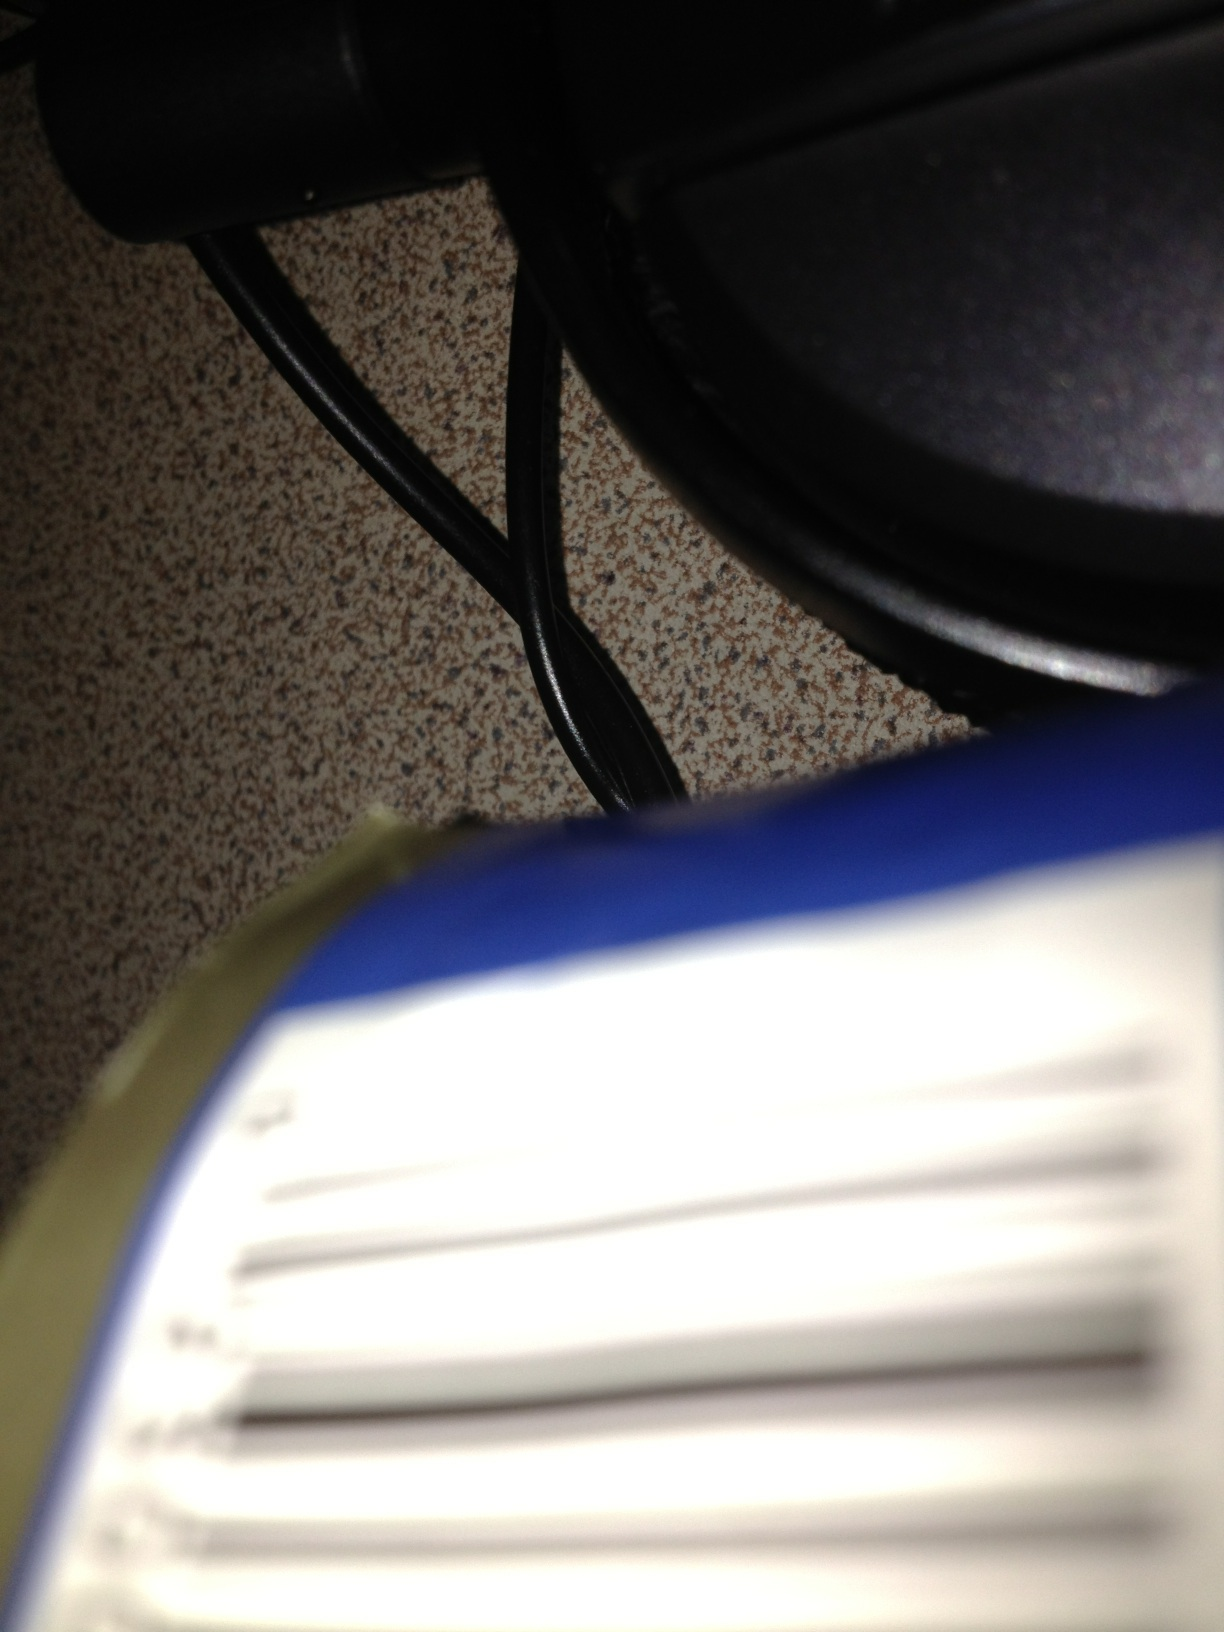
\includegraphics[width=0.3\textwidth]{img/vw_unans.jpg}

        \\
        & 
        & Q: What can is this?
        \end{tabular}
        
        % \caption{Triathlon results}
    \end{table}




\end{frame}

\begin{frame}
    \frametitle{VizWiz: Challenges and Possible Solutions}

    \begin{table}
        \begin{tabular}{c | c}
        Occuluded & Long text in images\\
        \hline \hline
        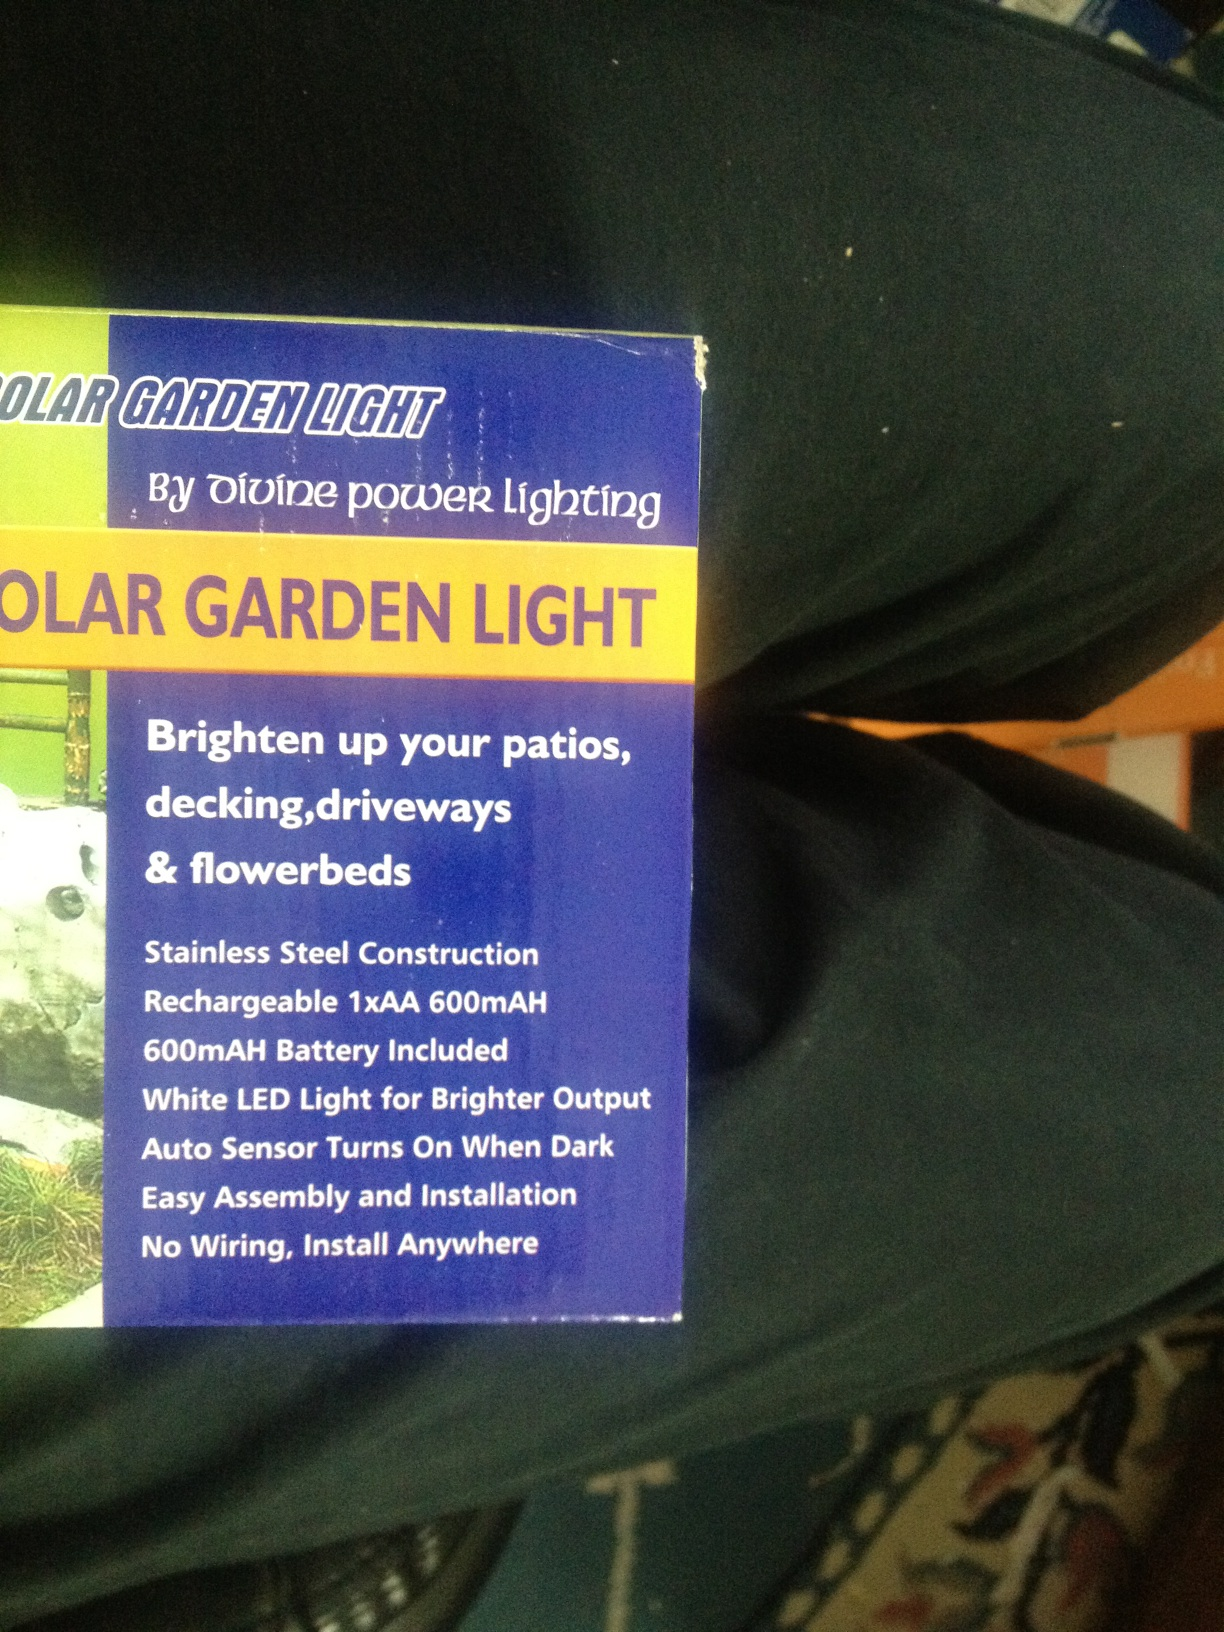
\includegraphics[width=0.3\textwidth]{img/vw_occ.jpg} & 
        
\includegraphics[width=0.3\textwidth]{img/vw_text.jpg}\\
        & Use text in image features extracted? 
        \end{tabular}
        % \caption{Triathlon results}
    \end{table}

    
    Working on
    \begin{itemize}
        \item Try to stats the answer distribution
        \item Extract visual features for images (use pretrained model from detectron2)
        \item Based on pytorch
    \end{itemize}

\end{frame}

\end{document}